\vspace*{\fill}
\begin{center}
	
\includegraphics[scale=0.7]{andre_profile}
\end{center}
\ \indent \emph{A interação com um contexto de negócio definido a partir de um processo a ser melhorado trouxe uma experiência distinta a qual achei bastante interessante para o contexto de requisitos de software, pois trouxe uma visão mais clara do limiar entre o contexto de negócio e o contexto da engenharia de requisitos.}
\\ \indent \emph{O contato com o time e os clientes diretamente e constantemente favorece muito as tomadas de decisão e trazem uma perspectiva mais descentralizada onde todos tem uma noção plena do estado atual do projeto, porém também é importante lembrar que esta situação pode levar a equipe a relevar prazos para uma organização mais favorável a sua atual situação.}
\\ \indent \emph{Em suma, o trabalho foi bem encaixado na disciplina e a interação entre as disciplinas foi muito proveitosa, assim como a relação entre os integrantes sempre foi boa, porém trago a sugestão de construção da solução através de um paradigma de programação mais flexível.}
\vspace*{\fill}

\newpage
\vspace*{\fill}
\begin{center}
	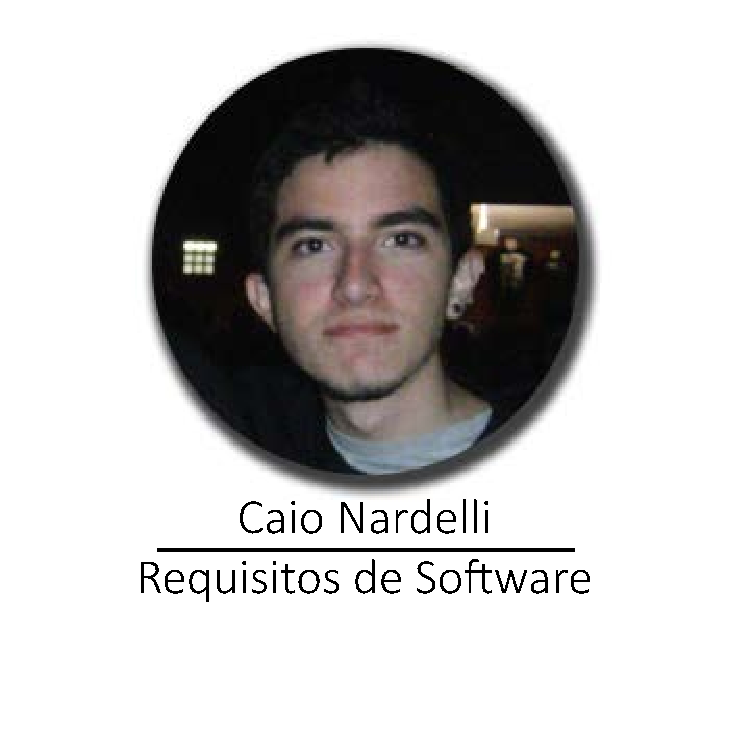
\includegraphics[scale=0.7]{caio_profile}
\end{center}
\ \indent \emph{No contexto desta disciplina de Requisitos de Software, notei que meu crescimento acadêmico foi substancialmente maior ao fazer o trabalho, do que simplesmente estudar teoria para uma prova.}
\\ \indent \emph{Aprendi que a organização e o trabalho em equipe são aspectos fundamentais para o sucesso de um projeto, e que só porque uma ferramenta gera uma solução diretamente pelo processo modelado, não quer dizer que é uma opção melhor.}
\vspace*{\fill}

\newpage
\vspace*{\fill}
\begin{center}
	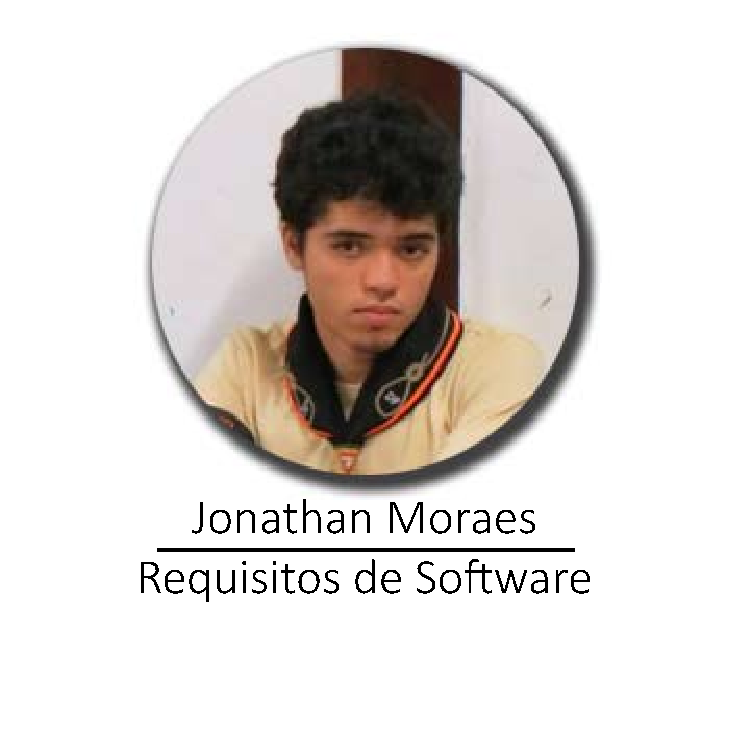
\includegraphics[scale=0.7]{jh_profile}
\end{center}
\vspace*{\fill}
\ \indent \emph{Pude observar com maior afinco as peculiaridades da engenharia de requisitos, onde tornou-se claro para mim a importância de se levantar requisitos com qualidade, gerenciar com eficiência e destreza e interagir com o cliente de forma objetiva e coesa. Ademais, estudar requisitos do ponto de vista do contexto ágil foi uma experiência gratificante, onde busco aplicar nos projetos do meu cotidiano, até mesmo fora do contexto de produção de software.}
\\ \indent \emph{Com o desenvolvimento de um projeto real (mesmo que o contexto seja fictício, todo o desenvolvimento do processo e da execução do mesmo foram feitos buscando o maior teor de profissionalismo possível), aprendi a me adaptar às mudanças, identificar necessidades e otimizar a busca por soluções plausíveis e condizentes com o contexto do negócio.}
\\ \indent \emph{De ponto à considerar, a utilização da ferramenta BPMS foi menos produtiva do que desejei, onde por diversas vezes cogitei o quão mais eficiente seria utilizar uma linguagem de programação para gerar as soluções propostas nos requisitos. Ainda assim, a experiência conquistada ao lidar com uma plataforma totalmente nova e abstrata para mim, buscando com ela uma solução tangível, trouxe uma bagagem didática que até então desconhecia: é preciso sempre se dedicar aos estudos, e em projetos é imprencidível mensurar o esforço que deve ser gasto para adquirir conhecimentos necessários para o desenvolvimento, algo que não conseguimos mensurar com facilidade.}

\newpage
\vspace*{\fill}
\begin{center}
	
\includegraphics[scale=0.7]{mh_profile}
\end{center}
\ \indent \emph{A realização do trabalho, sem dúvidas, fomentou o conhecimento inerente ao campo de Requisitos de Software. Através dos aspectos teóricos passados em sala de aula e, a partir da apresentação de um contexto de negócio, foi possível correlacionar a teoria à prática, favorecendo ainda mais a assimilação dos conteúdos.}
\\ \indent \emph{No decorrer da realização do trabalho, foi possível constatar que a execução, nem sempre, ocorre conforme o planejado. Inúmeras vezes foram contempladas atualizações no cronograma. Adicionalmente, contatou-se que uma boa solução é obtida a partir de uma análise concisa dos problemas e necessidades.}
\\ \indent \emph{Basicamente, achei interessante a integração entre as disciplinas. Minha única sugestão de melhoria seria no tocante à apresentação da solução. Ao invés de ser BPMS, os alunos poderiam codificar a solução, visto que o Bizagi Studio apresenta muitas limitações (Banco de Dados).}
\vspace*{\fill}

\newpage
\vspace*{\fill}
\begin{center}
	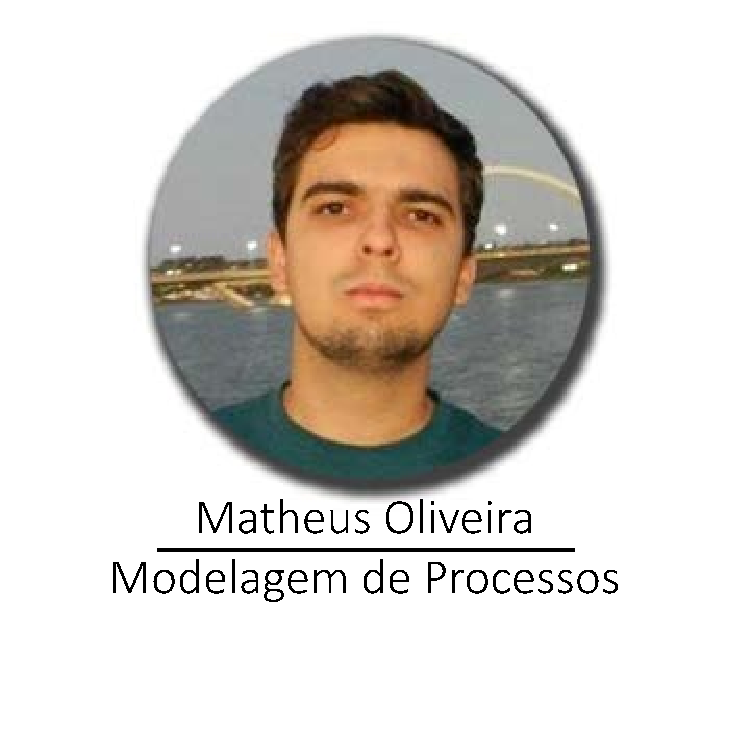
\includegraphics[scale=0.7]{mo_profile}
\end{center}
\ \indent \emph{Como relato de experiência, aprendi muito sobre como modelar um processo de maneira mais sequencial e menos complexa, de modo simplificado.}
\\ \indent \emph{De lições aprendidas: nomenclatura e simbologia na modelagem de processo, priorização de processos, identificação de problemas no processo.}
\\ \indent \emph{Como avaliação geral, acredito que a automação da solução poderia ser feita utilizando uma linguagem de programação convencional.}
\vspace*{\fill}

\newpage
\vspace*{\fill}
\begin{center}
	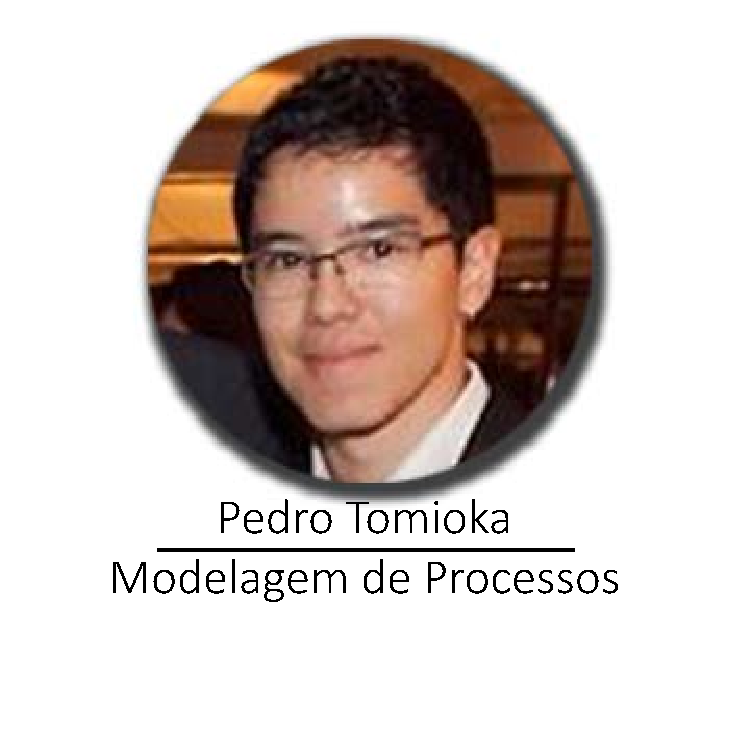
\includegraphics[scale=0.7]{pedro_profile}
\end{center}
\ \indent \emph{Como relato de experiência, aprendi como modelar, simular e propor uma melhoria para um processo de negócio.}
\\ \indent \emph{De lições aprendidas: o estudo do negócio deve ser feito com muito cuidado, considerando todos os stakeholders envolvidos e as restrições impostas por fatores internos e externos}
\\ \indent \emph{Como avaliação geral, as ferramentas de BPMS utilizadas para automação do processo TO-BE são muito confusas e difícil de mexer.}
\vspace*{\fill}
